Simulation and Code has attached to Homework(Q3\_b.m). For this $\beta$ we can find out that for 100 second all $J$ costs are zero and very near to zero so we neglect time after that.
\begin{figure}[H]
	\caption{System simulation for $\beta = 1000$}
	\centering
	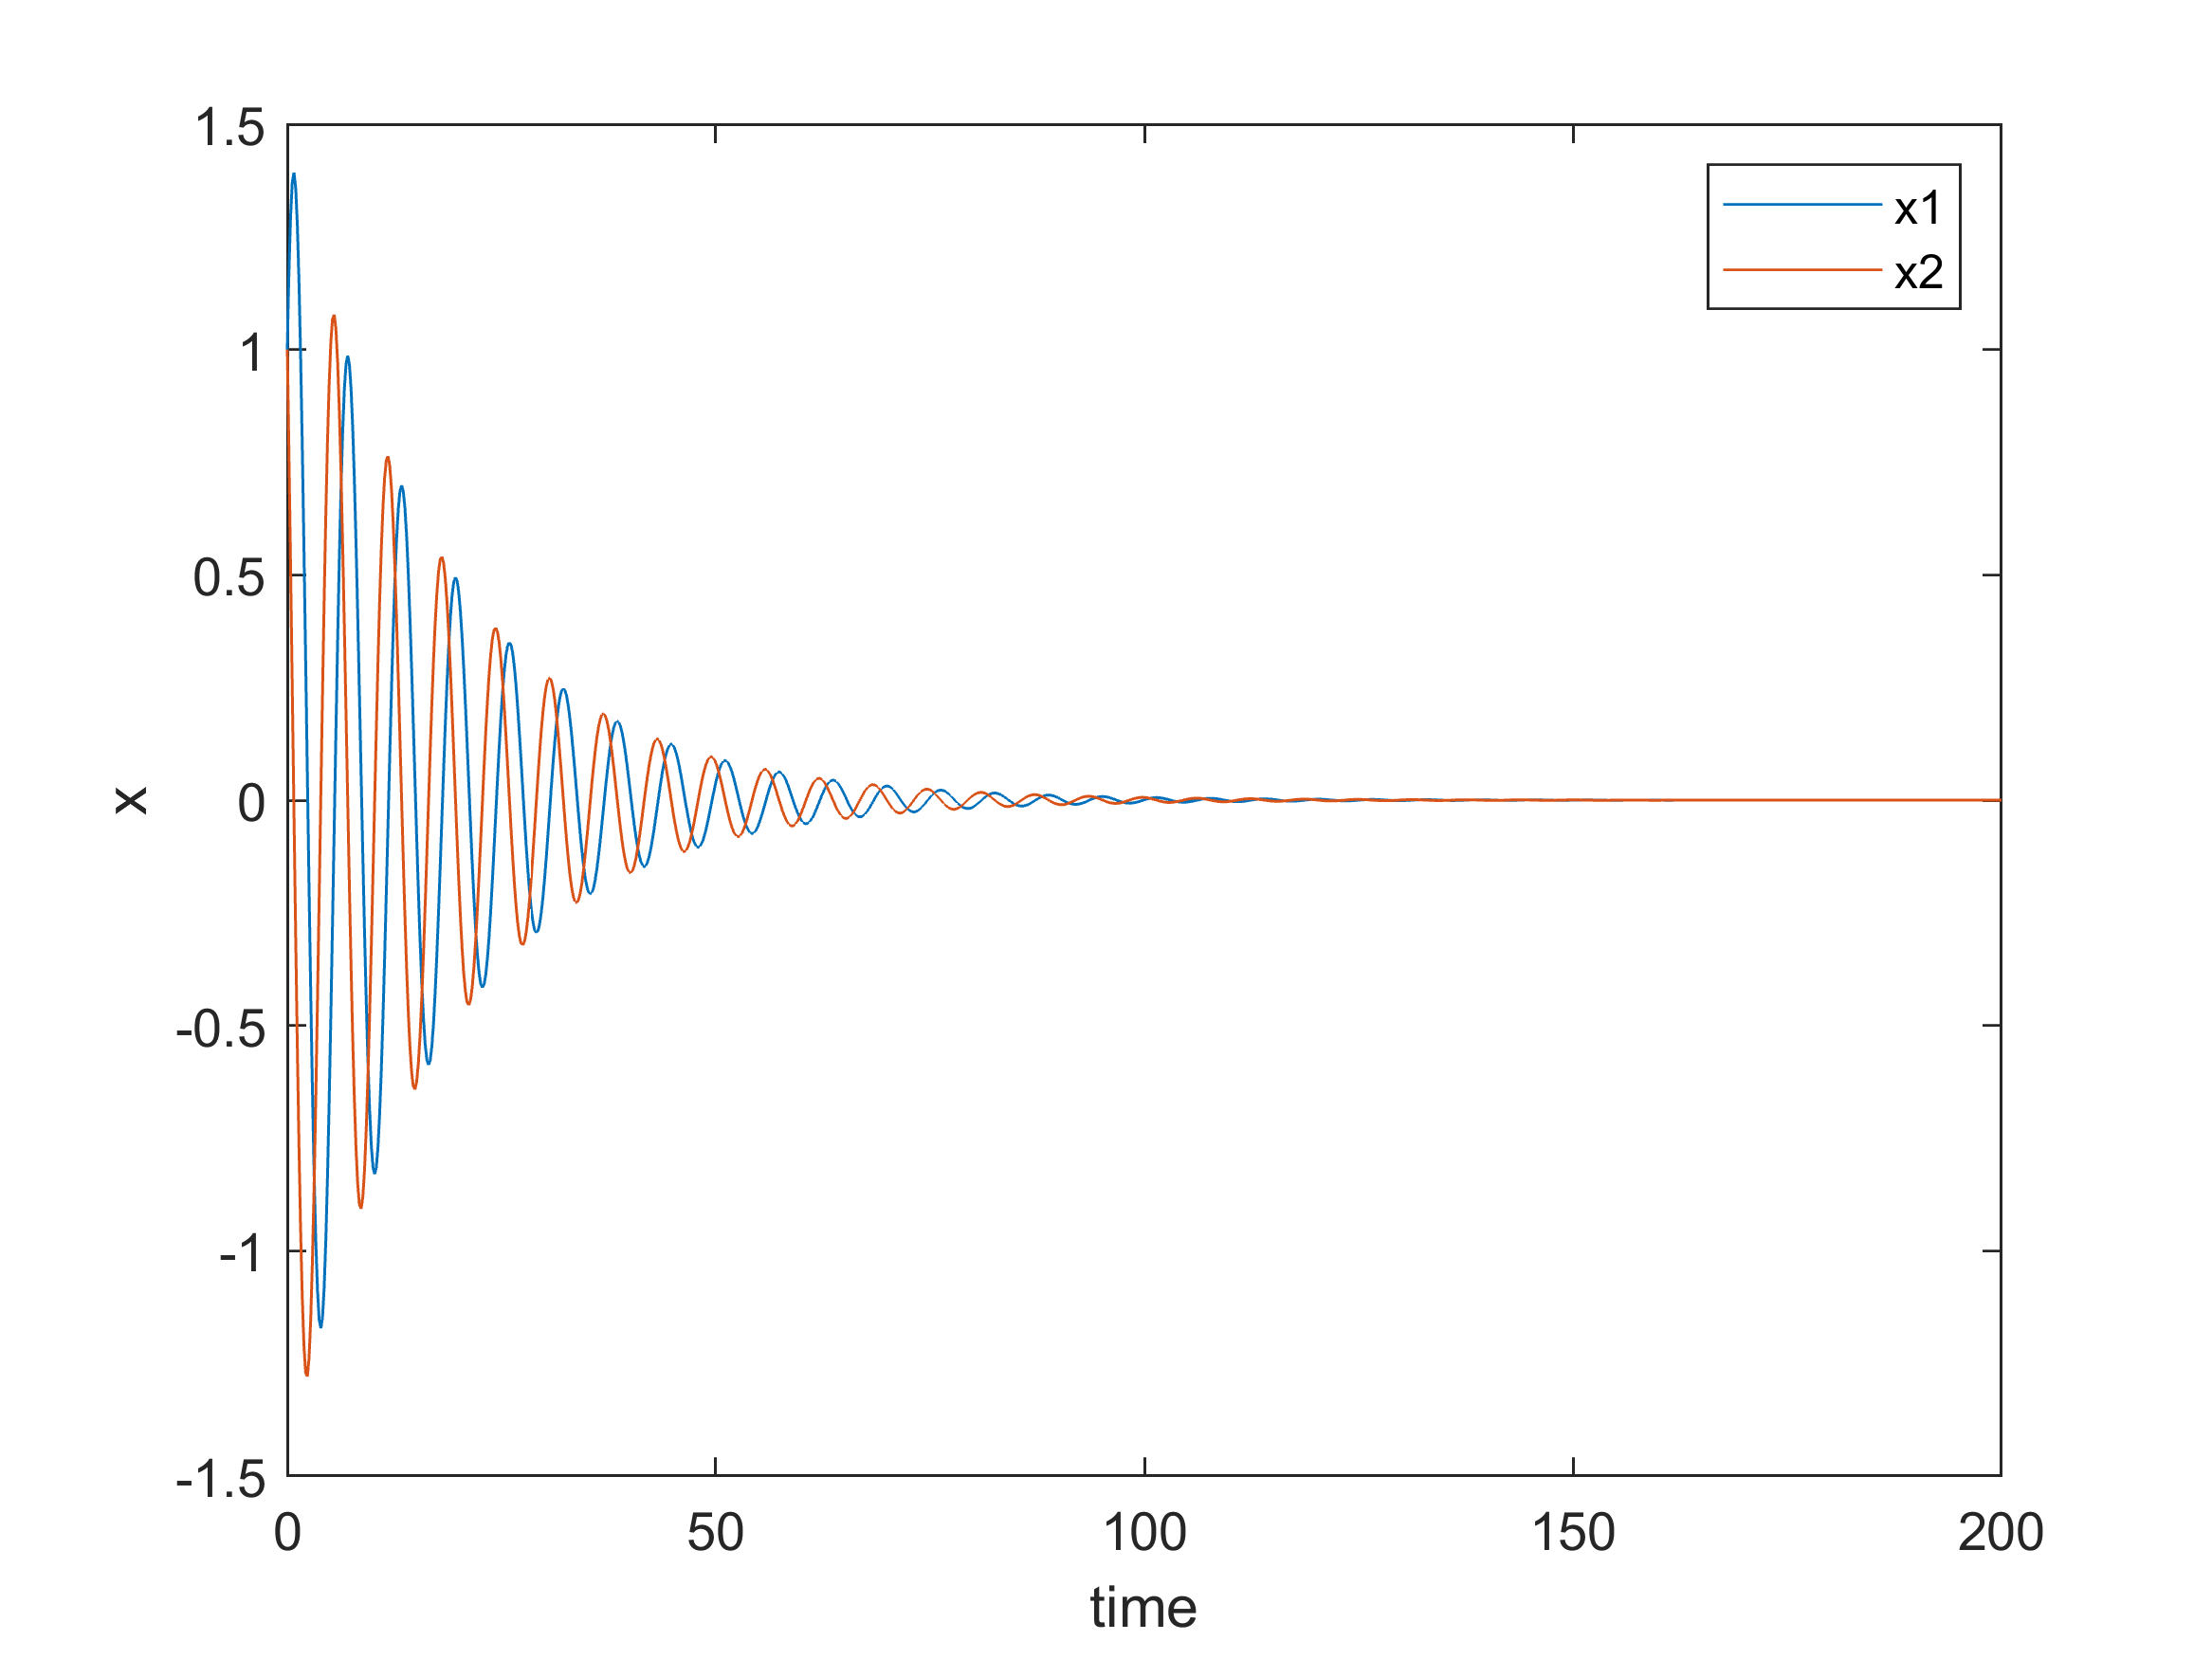
\includegraphics[width=12cm]{../Code/Q3/figures/FinalBeta.png}
\end{figure}
\newpage
\subsubsection{I}
$u(t)$ Cost:
$$J_u = \int_{0}^{\infty} u(t)^2d(t)$$
\begin{figure}[H]
	\caption{$u(t)$ cost in different $\beta$}
	\centering
	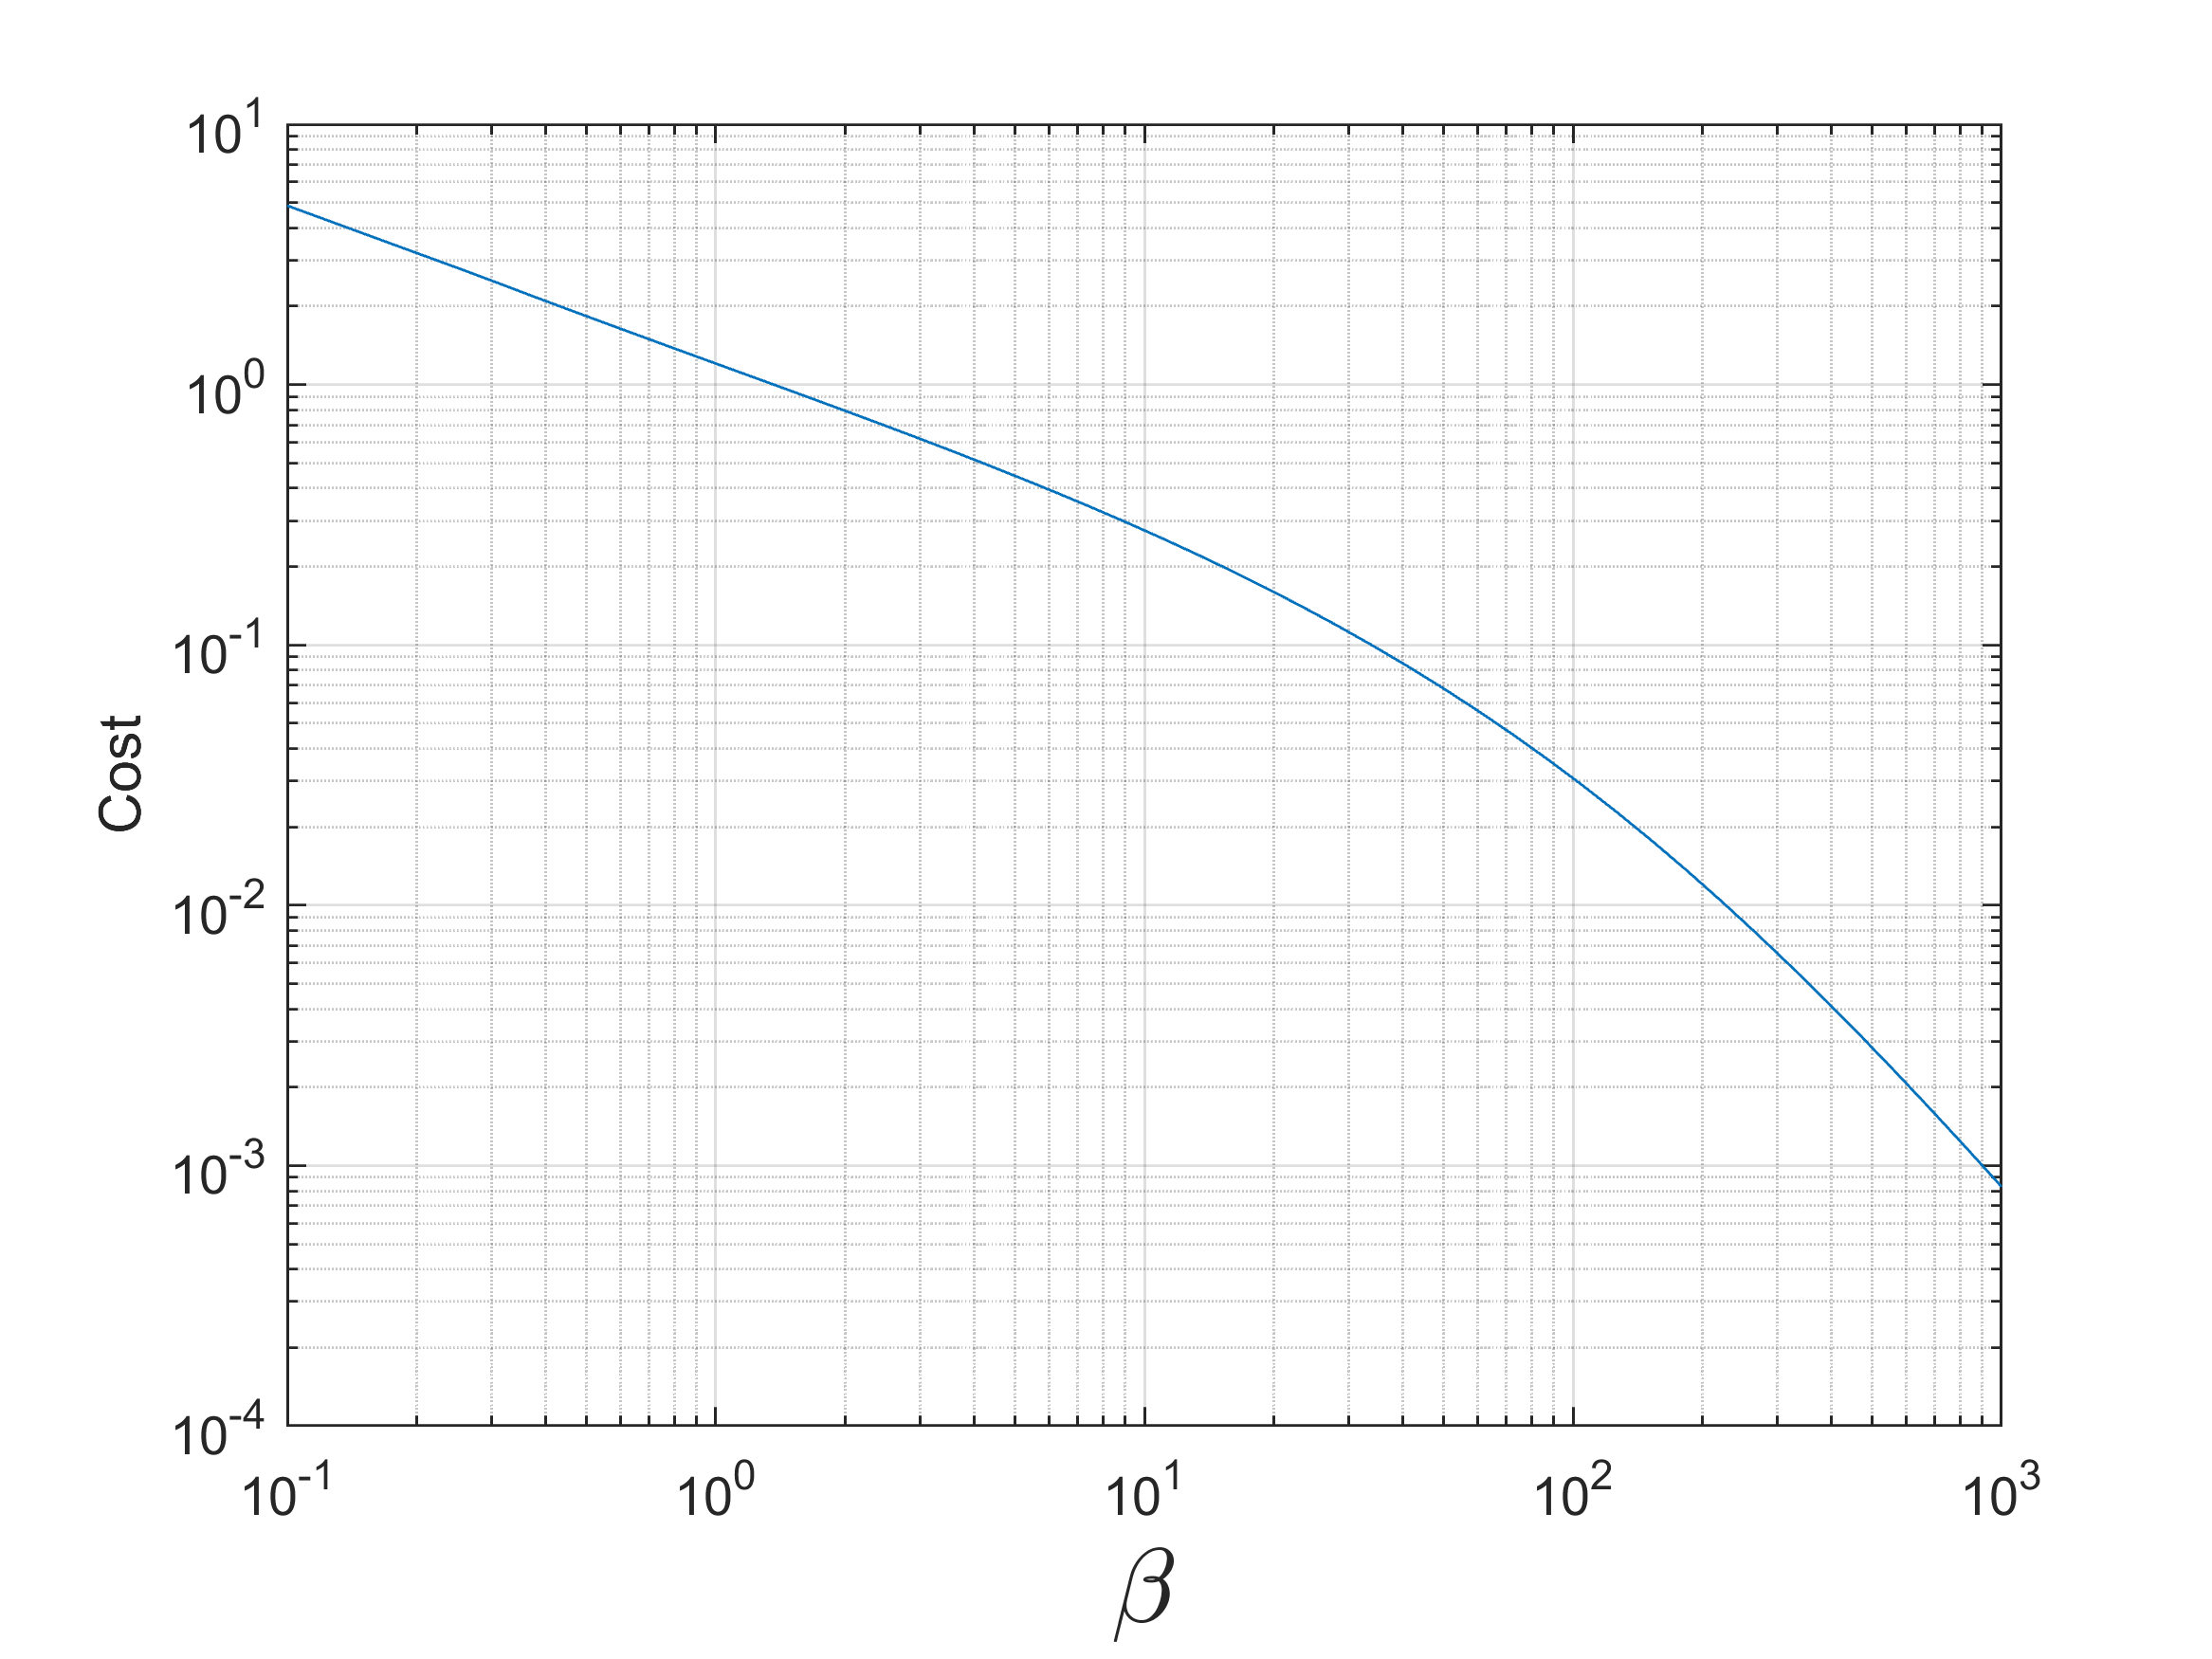
\includegraphics[width=12cm]{../Code/Q3/figures/uCost.png}
\end{figure}
\newpage
\subsubsection{II}
$x_1^2 + \dot x_2^2$ Cost:
$$J_u = \int_{0}^{\infty} (x^2 + \dot{x}^2)d(t)$$
\begin{figure}[H]
	\caption{$x^2 + \dot{x}^2$ cost in different $\beta$}
	\centering
	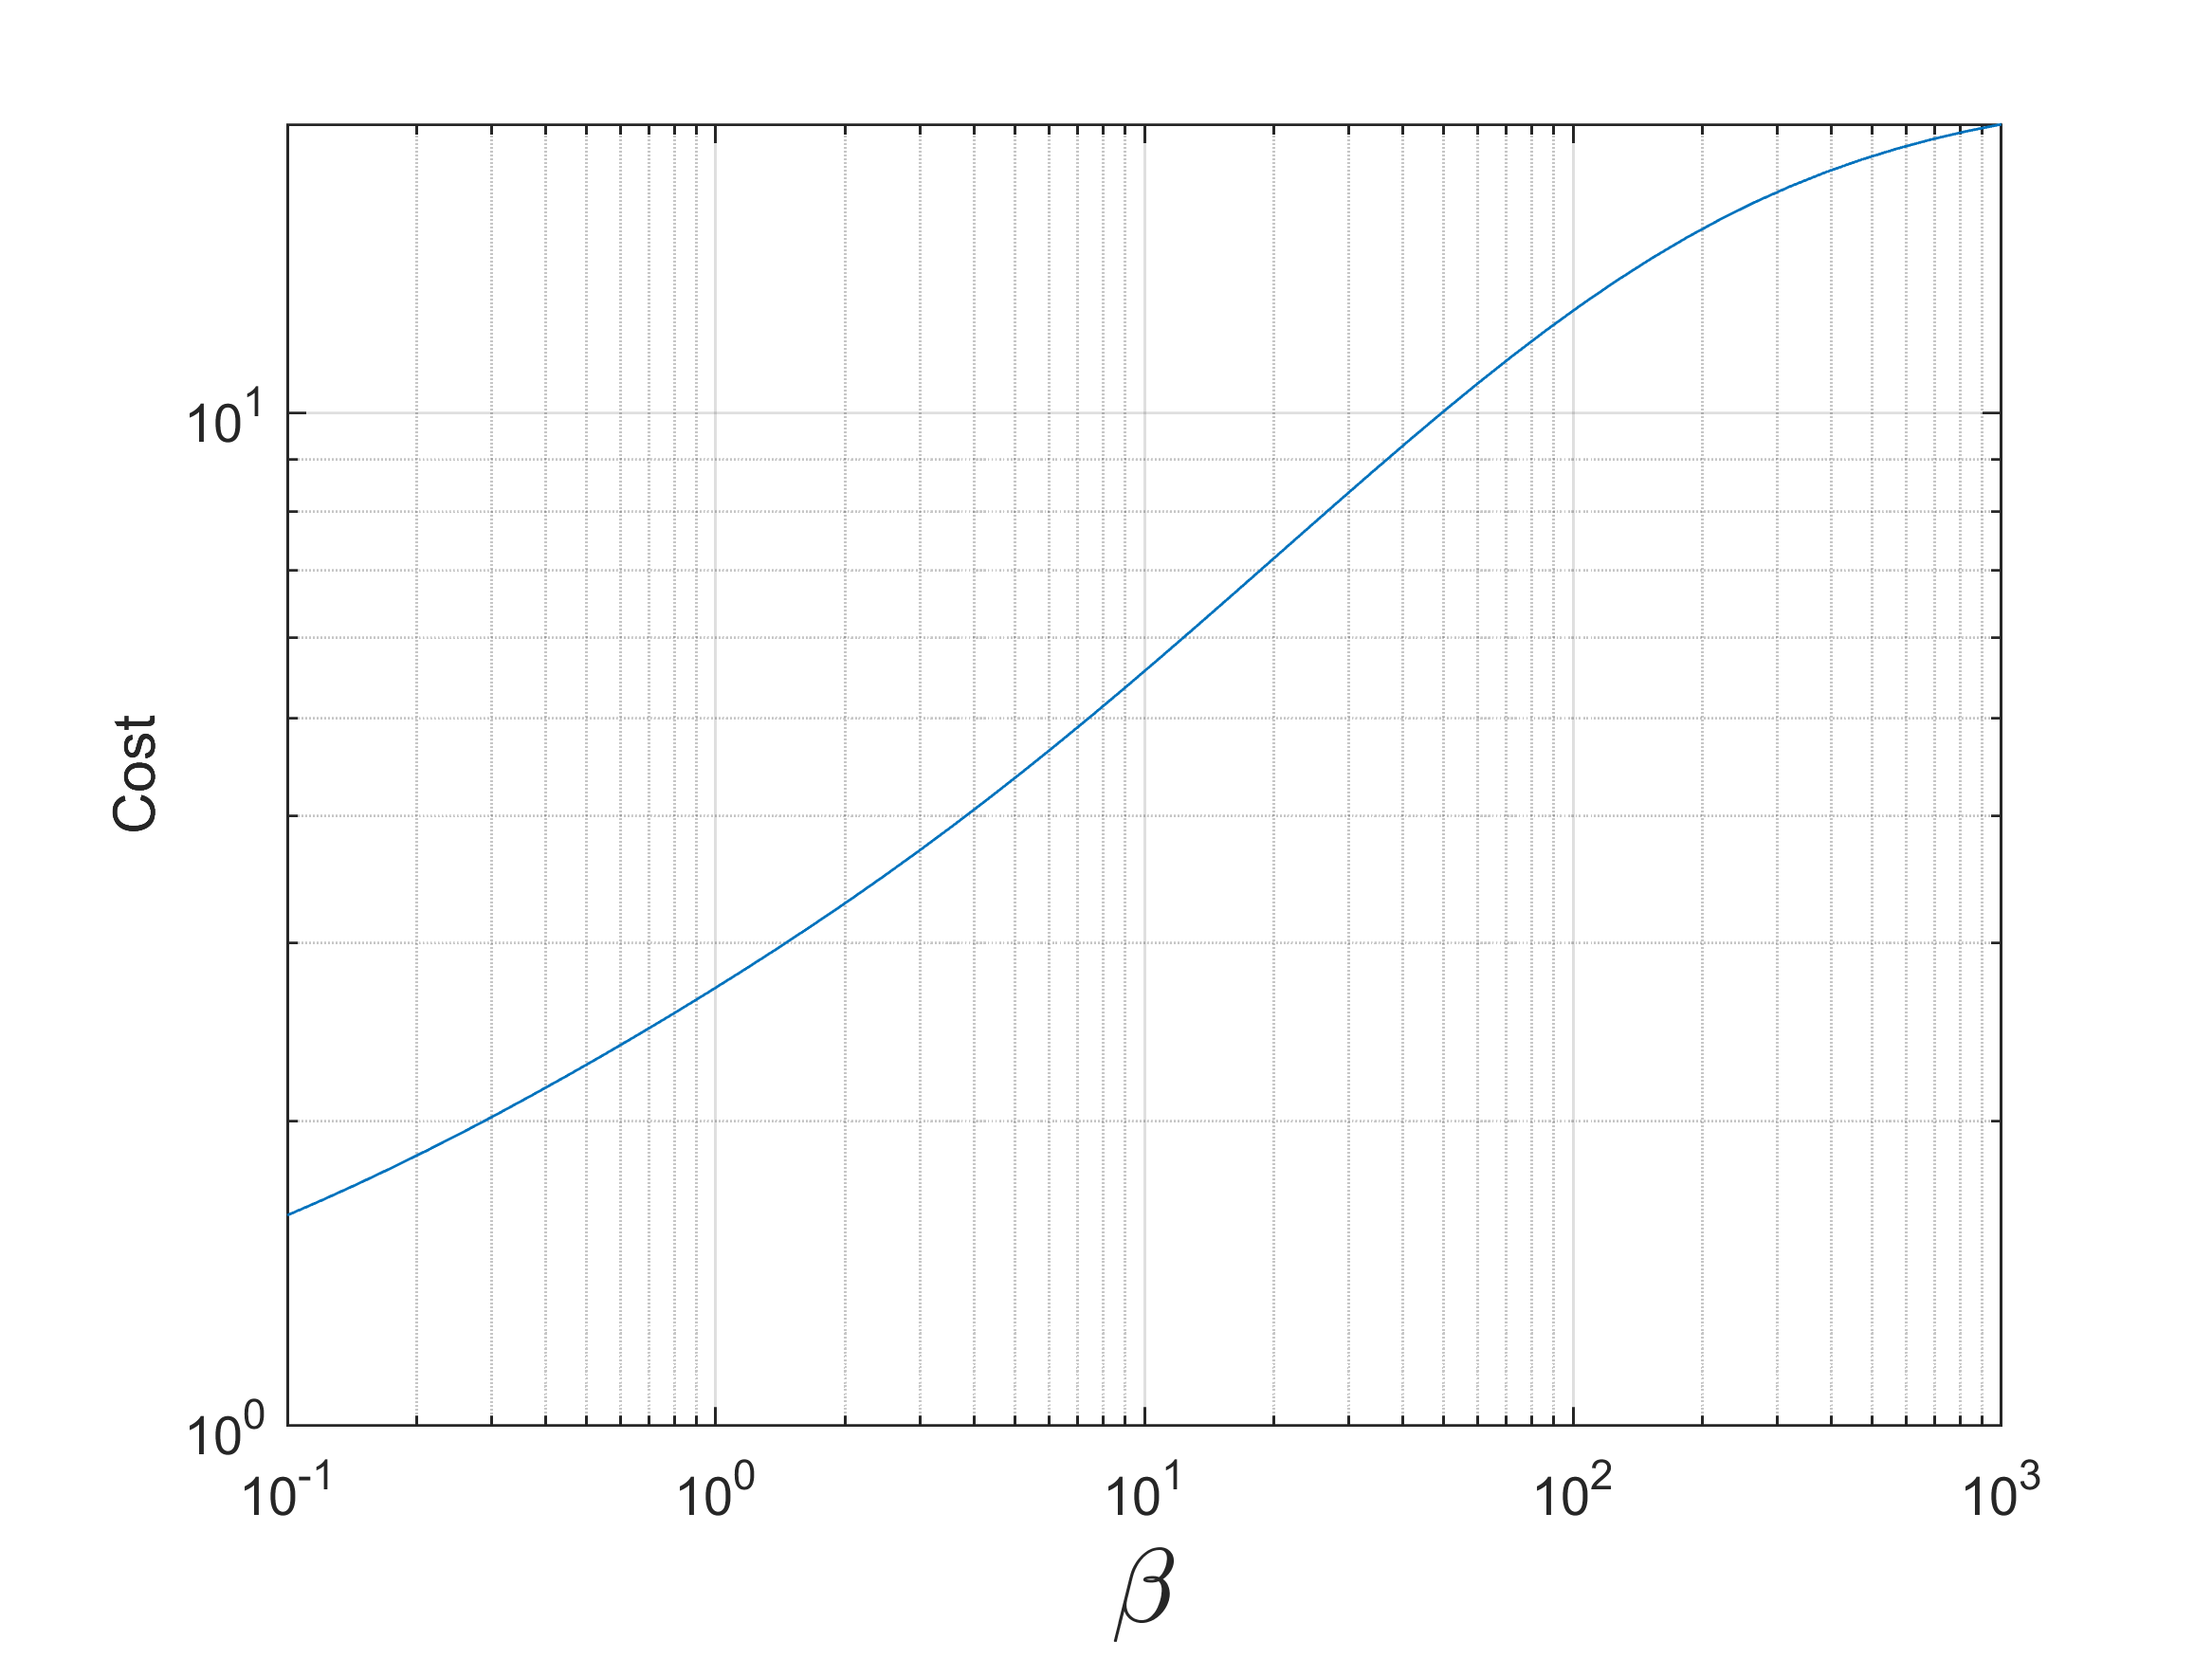
\includegraphics[width=12cm]{../Code/Q3/figures/xCost.png}
\end{figure}